\section{Components}
Chapter \ref{cha:technologies} examined the various components viable for use in the nodes. This section contains the decisions made regarding the components.

\subsection*{Arduino - sensor node}
%Explain the usage of Arduino Mega
Both Arduino Uno and Mega are used in the solution, as they qualify regarding specifications, and due to their availability to the project group. The Mega boards are not faster than the Uno boards, but can contain more program code and have more digital pins available. While the solution should be runnable on the Arduino Uno boards, the solution is restricted to the Uno's capacity and extra memory and pins on the Mega boards are superfluous. The Mega boards are still used in the project, not because of the extra functionality, but to enable the project group to test a larger system of nodes.

\subsection*{Raspberry Pi - main node}
The Raspberry Pi B+ model is used in the solution as the main node, based on the need to store, handle, and present data. This device has the responsibility of displaying the user interface, as well as processing and presenting the data received from the sensor nodes, as it has more processing power than the Arduinos, as well as the port needed to add a screen.


\begin{figure}[!h]
	\centering
	\makebox[\textwidth][c]{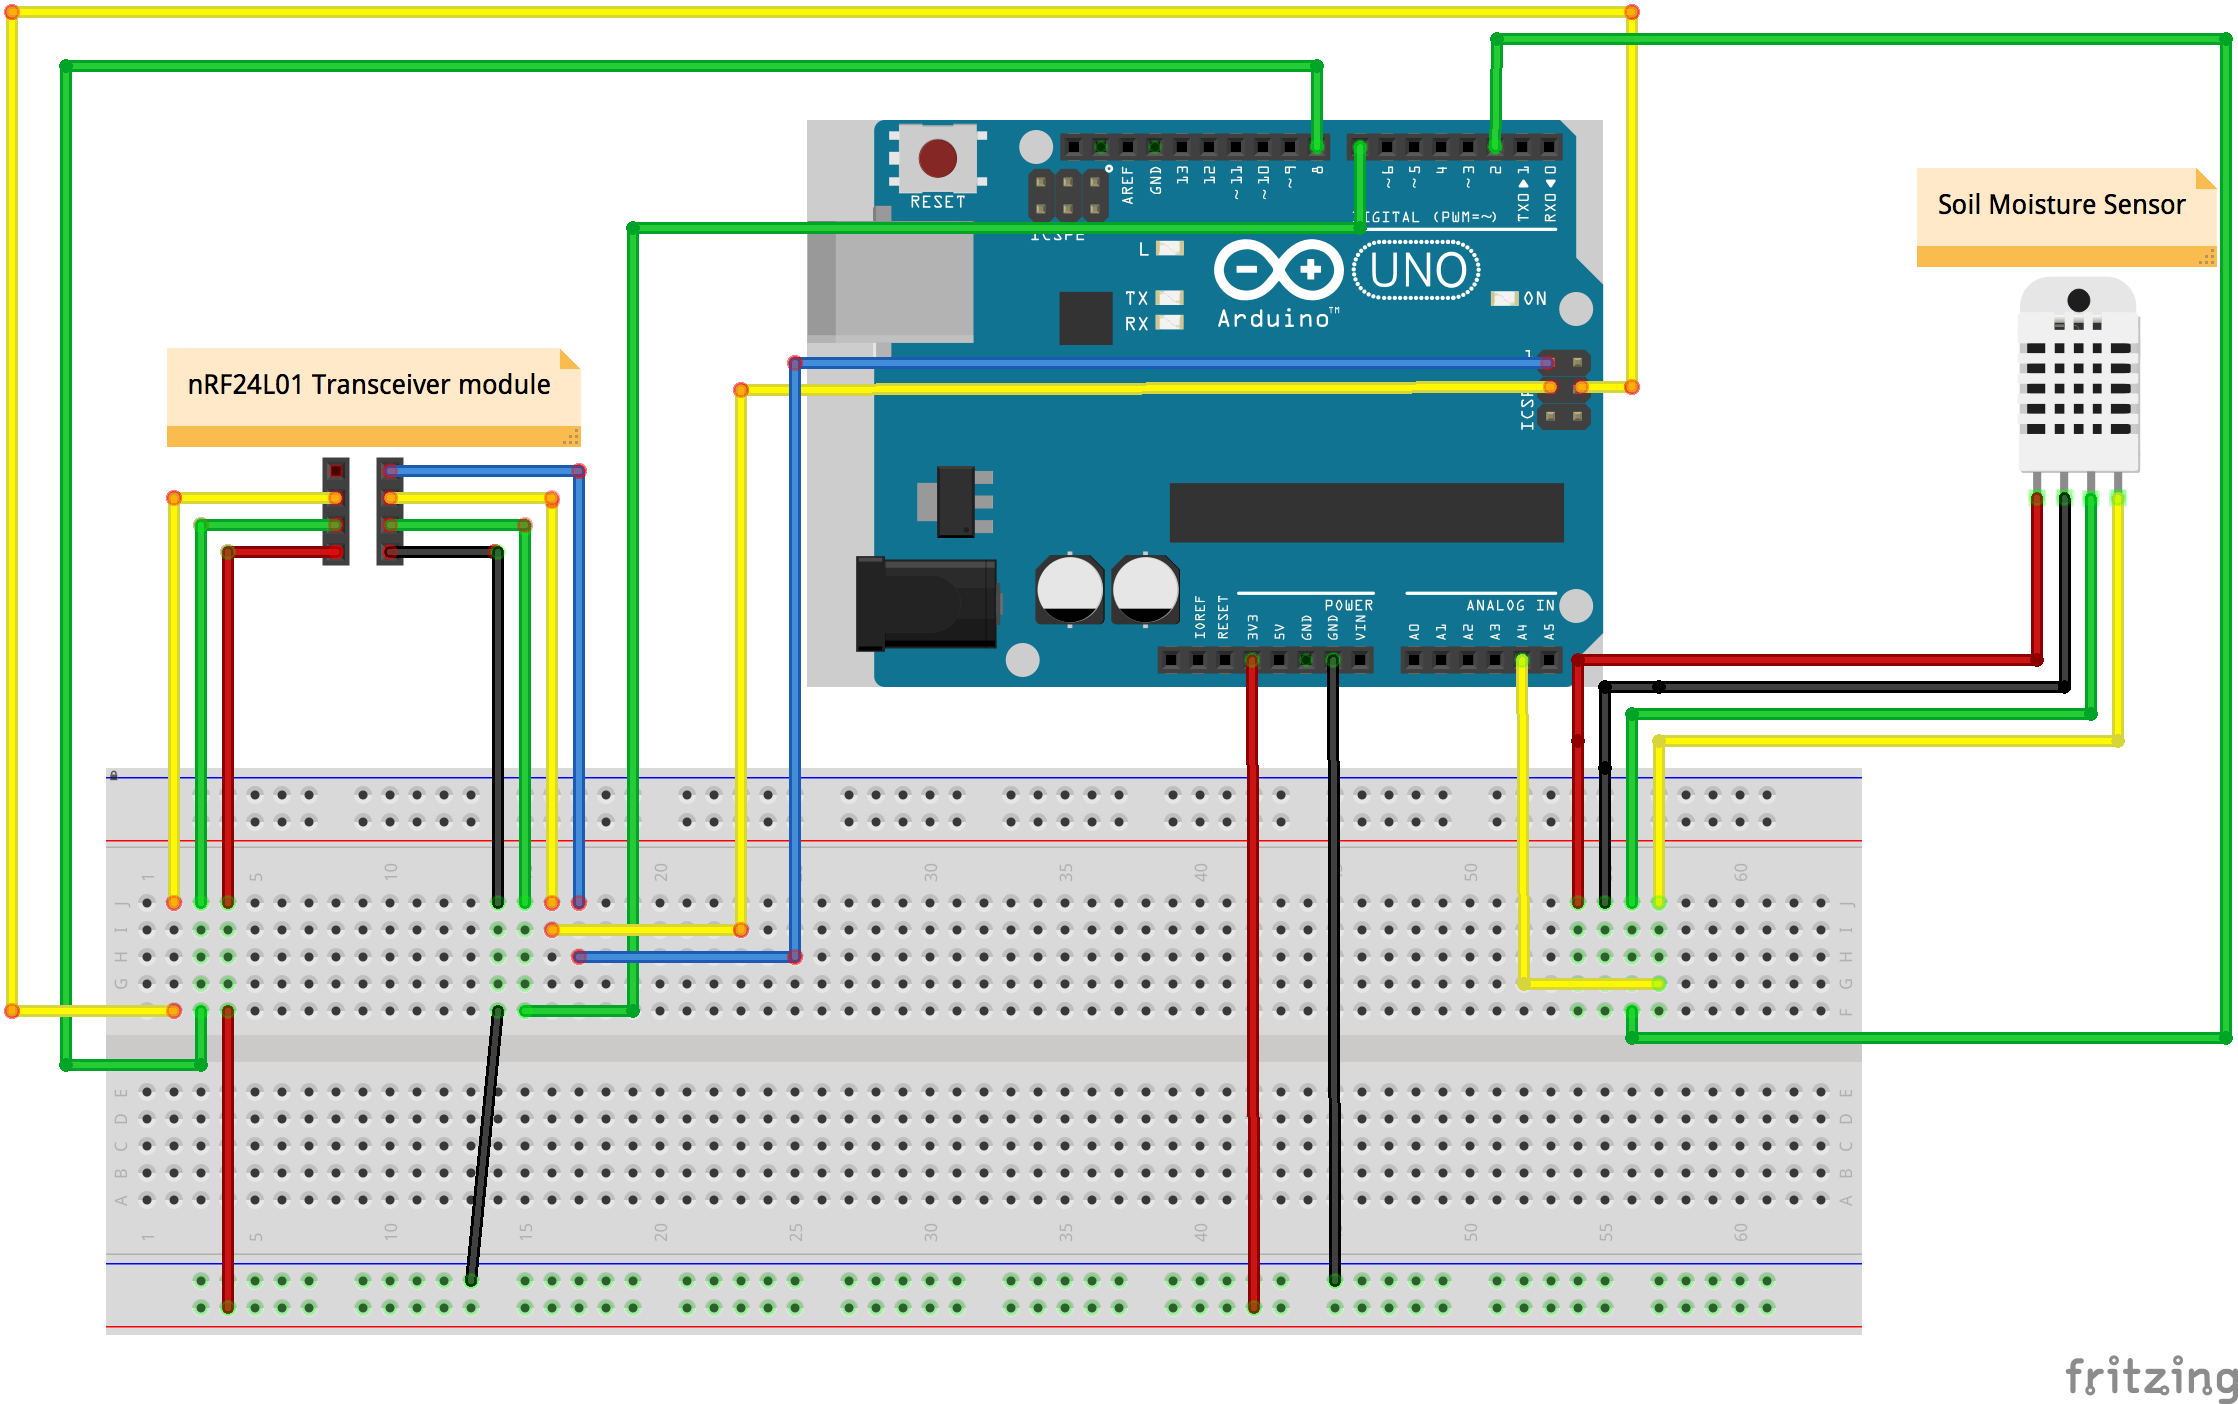
\includegraphics[width=1\textwidth]{chapters/design/figures/Sketch_bb.png}}
	\caption{Arduino connected to sensor and radio module.}
	\label{fig:compsketch}
\end{figure}

\subsection{nRF24L01 Transceiver}
The communication device chosen for this project is the nRF24L01, because of its documentation, price, and low power consumption. The transfer speed of the module is sufficient to send the small data packets, which makes this module good for the solution described in this report.

The nRF24L01 module contains multiple features for detecting packets loss. These includes checking hashes and sending acknowledgments\cite{nf24datasheet}. These features makes it harder to replace the radio modules in the nodes, as they are platform specific to the nRF24L01. The analysis examined the possibility of using different radio modules in case some requirements changes, which is not possible if using platform specific features. These features also causes more battery usage, which is a problem in devices being buried, as discussed in chapter \ref{cha:batcons}.

Based on this, these features have been disabled, which means that the radio packets does not contain a hash, nor does it send the default acknowledgments when packets arrives. The speed and power have also been turned down, so the device will transfer slower, and use less battery power.

\begin{figure}[!h]
	\centering
	\makebox[\textwidth][c]{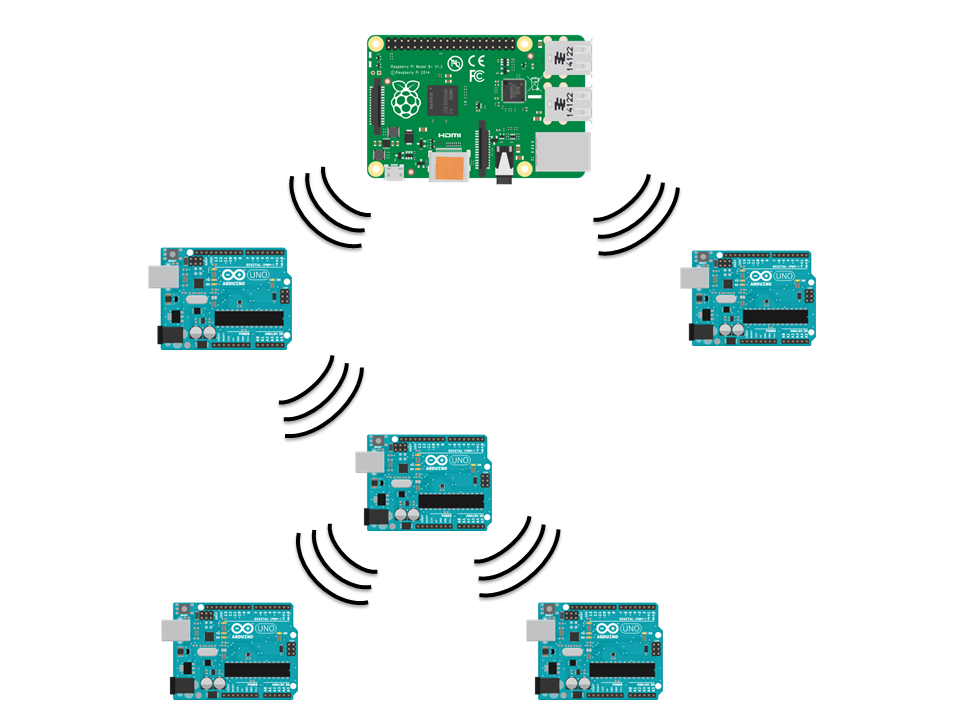
\includegraphics[width=1\textwidth]{figures/Raspberry-Arduino-Tree.png}}
	\caption{Raspberrry Pi main node and Arduino Uno sensor nodes wirelessly connected in a tree.}
	\label{fig:raspbuinoTree}
\end{figure}

\subsection*{Network of components}

With the components chosen and the data sheet for the nRF24L01 examined \cite{nf24datasheet}, the sensor nodes will be assembled as seen on figure \ref{fig:compsketch}.

\figref{raspbuinoTree}.\todo{Er disse brugt nogle steder?}



